
\documentclass[conference]{IEEEtran}
\usepackage{stmaryrd}
\usepackage{multirow}
\usepackage{amsfonts}
\usepackage{array}
\usepackage{color}

\usepackage{subfig}
\usepackage{epsfig}
\usepackage{chngpage}
\usepackage{graphicx}
\usepackage{cite}
\usepackage{arydshln,amssymb,color}
\usepackage{algorithm}
\usepackage{algorithmic}
\usepackage{flushend}
\usepackage{rotating}
\usepackage{amsmath}
% If the IEEEtran.cls has not been installed into the LaTeX system files,
% manually specify the path to it: e.g.,
% \documentclass[conference]{../sty/IEEEtran}

\usepackage{graphicx,times,epsfig,amsmath} % Add all your packages here

% correct bad hyphenation here
\hyphenation{op-tical net-works semi-conduc-tor IEEEtran}

\IEEEoverridecommandlockouts    % to create the author's affliation portion
                % using \thanks

\textwidth 178mm    % <------ These are the adjustments we made 10/18/2005
\textheight 239mm   % You may or may not need to adjust these numbers again
\oddsidemargin -7mm
\evensidemargin -7mm
\topmargin -6mm
\columnsep 5mm

\begin{document}


% paper title: Must keep \ \\ \LARGE\bf in it to leave enough margin.
\title{\ \\ \LARGE Extending Distance-based Ranking Models\\ in Estimation of Distribution Algorithms\thanks{Josu Ceberio, Ekhine Irurozki  and Jose A. Lozano are with the Department of Computer Science and Artificial Intelligence, University of the Basque Country UPV/EHU, Donostia, Spain (email: \{josu.ceberio, ekhine.irurozqui, ja.lozano\}@ehu.es).}\thanks{Alexander Mendiburu is with the Department of Computer Architecture and Technology, University of the Basque Country UPV/EHU, Donostia, Spain (email: alexander.mendiburu@ehu.es).} \thanks{Thanks to everyone!}}

\author{Josu Ceberio, Ekhine Irurozki, Alexander Mendiburu \\and Jose A. Lozano  (\textit{Member,~IEEE})}

% avoiding spaces at the end of the author lines is not a problem with
% conference papers because we don't use \thanks or \IEEEmembership
% use only for invited papers
%\specialpapernotice{(Invited Paper)}

% make the title area
\maketitle

\begin{abstract}
Recently, probability models on rankings have been proposed in the field of estimation of distribution algorithms in order to solve permutation-based combinatorial optimisation problems. Particularly, distance-based ranking models, such as Mallows and Generalized Mallows under the Kendall's-$\tau$ distance, have demonstrated their validity when solving this type of problems. Nevertheless, there are still many trends that deserve further study. In this paper, we extend the use of distance-based ranking models in the framework of EDAs by introducing new distance metrics such as Cayley and Ulam. In order to analyse the performance of the Mallows and Generalized Mallows EDAs under the Kendall, Cayley and Ulam distances, we run them on a benchmark of 120 instances from four well known permutation problems.

The conducted experiments showed that there is not just one metric that performs the best in all the problems. However, the statistical test pointed out that Mallows-Ulam EDA is the most stable algorithm among the studied proposals.
\end{abstract}

% no key words

\section{Introduction}
In combinatorics, many optimisation problems are defined as "the way of arranging $n$ number of objects" such that a specific criterion is maximised (or minimised). 
Codified naturally as permutations, these problems, referred to as {\it permutation-based problems}, are a subset of NP-Complete combinatorial optimisation problems. Vehicle routing~\cite{Tsutsui_VR}, job scheduling~\cite{Hejazi04} or assignment problems~\cite{Burkard98} are some of the several examples that can be found in the literature. Due to their high complexity and relevance, permutation-based problems have been frequently addressed in the field of combinatorial optimization.

Among the wide variety of exact, heuristic and metaheuristic algorithms, Branch and Bound~\cite{Wang1995}, Constructive Heuristics~\cite{Glover01}, Local Search~\cite{Stutzle06}, Genetic Algorithms~\cite{larranaga99}, Ant Colony Optimization~\cite{Chira2009}, Particle Swarm Optimization~\cite{Tasgetiren20071930}, or Estimation of Distribution Algorithms (EDA)~\cite{ceberio11b,lozano05} are a few of the algorithms that have been proposed in the combinatorial optimisation literature.

In this paper, we are particularly interested in the development of EDAs~\cite{muhlenbein96,larra01a} for solving permutation-based problems. EDAs are a type of evolutionary algorithm that, based on machine learning techniques, learn at each iteration a probabilistic model from a set of candidate solutions in order to capture the most relevant information. By sampling the model, EDAs guide the search towards promising areas of the search space. Numerous papers have demonstrated the validity of EDAs when solving combinatorial optimisation problems~\cite{larra01a,lozano05,Pelikan06,santana00,Qingfu05,ceberio13c,santana2008}. Permutation-based problems, however, present a real challenge for EDAs, since in most cases, the typical compact and factorized probability models cannot capture the {\it mutual exclusivity constraints} associated with permutations~\cite{huang2009}.

Recently, a number of papers have proposed using probability models on rankings in the framework of EDAs~\cite{ceberio11c,ceberio13a,ceberio13b, aledo2013}. Ceberio et al.~\cite{ceberio11c} published the first attempt of using probability models on rankings in the framework of EDAs. In that work, a {\it distance-based ranking model} called Mallows model (MM)~\cite{mallows,diaconis1988group,gMallows,Critchlow1991294} was used. This model, defined by two parameters, a central permutation $\sigma_0$ and a spread parameter $\theta$, is analogous to the Gaussian distribution over the domain of permutations. As an extension to the MM, the Generalized Mallows EDA was presented in~\cite{ceberio13a}. Proposed for the first time by Fligner et al.~\cite{fligner1988}, the Generalized Mallows model (GMM) is defined by a central permutation $\sigma_0$ and a vector of $n-1$ spread parameters $\boldsymbol{\theta}$, each of which affect a particular component of the solution.

The MM and the GMM assign to each permutation in the search space a probability that decays exponentially with respect to its distance to $\sigma_0$. Commonly,  the Kendall's-$\tau$ metric is the distance used to learn and sample these models~\cite{ceberio11c,ceberio13a}. Nevertheless, there exist other distance metrics that could be studied beyond the Kendall's-$\tau$~\cite{Critchlow1991294}. In this sense, with the aim of exploring other possibilities, in this paper we extend previous works by introducing efficient implementations of the Mallows and Generalized Mallows models for the Cayley~\cite{irurozki2013a} and Ulam~\cite{irurozki2013b} distances. 

In order to study the performance of the Kendall's-$\tau$, Cayley and Ulam metrics in the Mallows and the Generalized Mallows EDAs, we test these algorithms on a benchmark of 120 instances from the Traveling Salesman Problem (TSP), the Quadratic Assignment Problem (QAP), the Linear Ordering Problem (LOP) and the Permutation Flowshop Scheduling Problem (PFSP). The conducted experiments show that there is not just one algorithm that performs the best in all the proposed instances. However, the statistical analysis concluded that the Mallows EDA under Ulam distance is the preferred algorithm due to its stable performance in all the problems. In addition, the experiments reveal that Mallows EDA under Cayley is the algorithm that performs the worst.

The remainder of the paper is organised as follows: in the next section, the permutation problems considered in the experimental study are briefly introduced. Afterwards, in Section~\ref{sec:models} the Mallows and the Generalized Mallows models are described in detail. In Section~\ref{sec:metrics}, Kendall's-$\tau$, Cayley and Ulam distances are introduced, and their respective learning and sampling procedures are detailed. In Section~\ref{sec:experiments}, an experimental study of the Mallows and the Generalized Mallows EDAs under the different distance metrics is performed. Finally, some conclusions and ideas for future work are presented in Section~\ref{sec:conclusions}.

\section{Permutation-based Combinatorial Optimization Problems}\label{sec:problems}

Permutation-based problems are combinatorial optimization problems whose solutions can be naturally represented as a permutation. A permutation is understood as a bijection  $\sigma$ of indexes $\{1,\ldots,n\}$ onto $\{1,\ldots,n\}$, where $\sigma(i)$ (also denoted as $\sigma_i$)\footnote{With readability purposes we will use $\sigma(i)$ and $\sigma_i$ interchangeably throughout the paper.} denotes the item at position $i$, and $\sigma^{-1}(i)$ stands for the position of item $i$ in $\sigma$ (denoted also as $\sigma\langle i \rangle$).

In what follows, we briefly describe the problems we consider in this paper. 

\subsection{Linear Ordering Problem}

Given a matrix $B = [b_{ij}]_{n \times n}$ of numerical entries, the Linear Ordering Problem (LOP)~\cite{marti2011linear,ceberio14a} consists of finding a simultaneous permutation $\sigma$ of the rows and columns of $B$ such that the sum of the entries above the main diagonal is maximised (or equivalently, the sum of the entries below the main diagonal is minimised). The equation below formalises the LOP function: \[f(\sigma)=\sum_{i=1}^{n-1} \sum_{j=i+1}^n b_{\sigma_i\sigma_j}\]where $\sigma_i$ denotes the index of the row (and column) located at position $i$ in the solution $\sigma$.  A particular feature of this problem worth noting is that the contribution of an index $\sigma_i$ to the objective function depends on the previous and posterior sets of indexes, but not on their relative ordering~\cite{ceberio14a}.
 
\subsection{Permutation Flowshop Scheduling Problem}

In the permutation flowshop scheduling problem (PFSP)~\cite{baker1974}, $n$ jobs $(i=1,\ldots,n)$ have to be scheduled on $m$ machines $(j=1,\ldots,m)$ in such a way that a given criterion is minimized.
A job consists of $m$ operations and the $j$-th operation of each job must be processed on machine $j$ for a given specific processing time without interruption. The processing times are fixed, non-negative values and every job is available at time zero. At a given time, a job can start on the $j$-th machine when its $(j-1)$-th operation has finished on machine $(j-1)$, and machine $j$ is free. A solution for the problem is codified as a permutation $\sigma$ of length $n$ where $\sigma_i$ denotes the job at position $i$.

With respect to the optimisation criterion, we considered the total flow time (TFT), which optimises the sum of the completion times of each job. Eq.~\ref{E:objective1} expresses mathematically the concept of TFT for a solution $\sigma$, where $c_{\sigma_i,m}$ stands for the completion time of job $\sigma_i$ on machine $m$.
\begin{equation}
F(\sigma)=\sum_{i=1}^n c_{\sigma_i,m}
\label{E:objective1}
\end{equation}
Being $p_{\sigma_i,j}$ the processing time required by job $\sigma_i$ on machine $j$, the completion time of job $\sigma_i$ on machine $j$ can be recursively calculated as:
\begin{equation*}
\scalebox{0.9}{$c_{\sigma_i,j}=$}
\begin{cases} 
\scalebox{0.9}{$p_{\sigma_i,j}$} & \scalebox{0.8}{$i = j = 1$}\\
\scalebox{0.9}{$p_{\sigma_i,j} + c_{\sigma_{i-1},j}$} & \scalebox{0.8}{$i > 1, j = 1$}\\
\scalebox{0.9}{$p_{\sigma_i,j} + c_{\sigma_i,j-1}$} & \scalebox{0.8}{$i = 1, j > 1$}\\
\scalebox{0.9}{$p_{\sigma_i,j} + \max\{c_{\sigma_{i-1},j},c_{\sigma_i,j-1}\}$} & \scalebox{0.8}{$i > 1, j > 1$}
\end{cases}
\label{E:completion1}
\end{equation*}
Note that the completion time of each job $\sigma_i$ depends on the ordering of the previous $\{\sigma_1,\ldots,\sigma_{i-1}\}$ jobs, and therefore the contribution of each job is highly determined by its processing times as well as by the ordering of the previously scheduled jobs.

\subsection{Traveling Salesman Problem}
The Traveling Salesman Problem (TSP)~\cite{DBLP:conf/icga/GoldbergL85} consists of looking for the shortest path, in terms of time, distance, or any similar criterion, to go over $n$ different cities visiting each city only once and returning to the city of departure. A solution for the problem is codified as a permutation $\sigma$ of cities where $\sigma_i$ denotes the city visited in the $i$-th position. The objective function $f$ is defined as the sum of the distances of going from city $i-1$ to $i$, denoted as $d_{ij}$, through all cities in the order specified in $\sigma$: \[f(\sigma)=\sum_{i=2}^n d_{\sigma_{i-1}\sigma_i} + d_{\sigma_n\sigma_1}\]
In the TSP we note that due to the cyclic nature of the solutions, the relevant information to calculate the fitness function of a solution $\sigma$ is given by the relative ordering of the cities in the permutation, and not by their absolute position, which in this case is irrelevant.

\subsection{Quadratic Assignment Problem}
The Quadratic Assignment Problem (QAP)~\cite{koopmans1955} is the problem of allocating a set of facilities to a set of locations, with a cost function associated to the distance and flow between the facilities. The objective is to assign each facility to a location such that the total cost is minimized. Specifically, given two $n \times n$ numerical matrices $H = [h_{ij}]$ and $D = [d_{ij}]$, where $h_{ij}$ is the flow between facility $i$ and facility $j$, and $d_{ij}$ denotes the distance between the location $i$ and $j$, the goal is to find a permutation $\sigma$ (where $\sigma_i$ represents the facility allocated at position $i$), such that the function \[f(\sigma)= \sum_{i=1}^n \sum_{j=1}^n h_{\sigma_i\sigma_j}*d_{ij}\]is minimised. In this problem, the quality of the solution depends on the absolute position of each facility in the permutation.   

\section{Mallows and Generalized Mallows models}
\label{sec:models} %-------------------------------------------------------------		MODELS
The Mallows model (MM)~\cite{mallows} is one of the most popular probability models for permutation spaces. Under this model, the probability value of every permutation $\sigma \in \mathbb{S}_n$ (where $\mathbb{S}_n$ stands for the set of $n!$ permutations of $n$ items) depends on just two parameters: a spread parameter $\theta$, and the distance to a central permutation $\sigma_0$, which is calculated by a particular metric $D(\sigma,  \sigma_0)$. Formally, the MM is defined as follows:
\begin{equation}
P(\sigma)= \psi(\theta)^{-1}exp(-\theta D(\sigma,\sigma_0)) 
\label{eq:mallows}
\end{equation}
\noindent 
where $\psi(\theta)$ is a normalization constant. When $\theta > 0$, the central permutation $\sigma_0$ is the mode of the distribution. The model assigns to each permutation $\sigma \in \mathbb{S}_n$ a probability that decays exponentially with respect to its distance to  $\sigma_0$. On the one hand, the larger the value of $\theta$, the more peaked the distribution becomes around the central permutation. On the other hand, when $\theta$ equals 0, Eq.~\ref{eq:mallows} assigns equal probability to every permutation $\sigma$ in $\mathbb{S}_n$, and for $\theta < 0$ then $\sigma_0$ is the antimode. 

As an extension to the MM, the Generalized Mallows model (GMM) was proposed in~\cite{fligner1988}. Under the GMM, the central permutation $\sigma_0$ is also the mode of the distribution. However, instead of a single spread parameter $\theta$, the GMM makes use of a vector of $n-1$ spread parameters $\boldsymbol{\theta}=(\theta_1, \theta_2, ... \, , \theta_{n-1})$, each $\theta_j$ affecting a particular position $j$ in the permutation.  This allows modelling a distribution with more emphasis on the consensus of certain positions of the permutation while having more uncertainty in some of the others. The  GMM  requires the metric to be decomposed into $n-1$ terms in such a way that it can be expressed as 
\begin{equation}
D(\sigma, \sigma_0)=\sum_{j=1}^{n-1}S_j(\sigma\sigma_0^{-1})
\label{eq:decomp}
\end{equation}
where $\sigma_0^{-1}$ stands for the inverse permutation of $\sigma_0$, $\sigma\sigma_0^{-1}$ denotes the composition operation between $\sigma$ and $\sigma_0^{-1}$ and $S_j(\sigma \sigma_0^{-1})$ is the term associated to the position $j$. For such a metric, the GMM model is formalised as
\begin{equation}
P(\sigma)= \psi(\boldsymbol{ \theta})^{-1} exp(\sum_{j=1}^{n-1}-\theta_j S_j(\sigma \sigma_0^{-1}))
\label{eq:gmallows}
\end{equation}

In order to introduce these models in the framework of EDAs, it is necessary to define efficient learning and sampling methods for each model-metric. As regards the learning, this process consists of two steps that are similar for all the model-metric combinations: first, given a sample of permutations, the consensus permutation $\sigma_0$ is calculated, and then, the spread parameter $\theta$ for MM (or $\boldsymbol\theta$ for GMM) is estimated. Usually, this process is approached via maximum likelihood estimation (MLE). However, the time required for an exact learning scales factorially with the number of items~\cite{ceberio13a,irurozki2013a,irurozki2013b}, and thus, in this work we carry out an approximate learning of the parameters:
\begin{enumerate}
\item The estimated consensus permutation $\hat \sigma_0$ is calculated as the {\it set median permutation}, which is the permutation in the sample that minimizes the sum of the distances to the rest of the permutations in the sample. Although one can find in the literature many approximation algorithms for the MLE for the consensus permutation~\cite{ali2011}, we have decided to use the set median permutation in this work for two reasons: (1) Computing the set median permutation is a quick process, carried out in time $O(dm^2)$, where $d$ denotes the time complexity of computing the distance between two permutations and $m$ the number of permutations in the sample. (2) Using the same approximation method for the consensus permutation for every distance metric, we try to compare the EDAs independently of the quality of the learning algorithm.

\item Once $\hat\sigma_0$ is estimated, the MLE for the spread parameter $\theta$ for MM (or $\boldsymbol \theta$ for GMM) is computed. The expression for this parameter is obtained by equaling to zero the derivative of the likelihood. This expression differs depending on the distance metric, however, we solved them by means of the Newton-Raphson algorithm. For further details we refer the interested reader to~\cite{irurozki2013c,ceberio13a}.
\end{enumerate}

As regards the sampling process, each metric has a particular procedure, and thus, in the next section we introduce the Kendall's-$\tau$, Cayley and Ulam metrics in detail, including the method for sampling (obtain a new permutation).

\section{Distance Metrics}\label{sec:metrics} %-------------------------------------------------------------		DISTANCEs
Due to its applications in preference modelling, Kendall's-$\tau$ metric is the metric that has captured the attention of the research community the most~\cite{Mandhani2009,Cheng2009,Caragiannis2013}. However, recently, new techniques for efficiently learning and sampling the MM and the GMM models for Cayley~\cite{irurozki2013a} and Ulam~\cite{irurozki2013b} distance metrics have been proposed. This fact has encouraged us to study the performance of the MM and the GMM under these three distance metrics inside the framework of EDAs.

%As previously mentioned, in this work we aim to compare Kendall's-$\tau$, Cayley and Ulam metrics metrics under the MM and GMM in the framework of EDAs, and thus, in what follows, the methods for learning and sampling the MM and the GMM for these metrics are detailed. Recall that the MM is the particular case of the GMM in which every $\theta_j$ have the same value. Therefore, unless otherwise stated, the expressions and procedures given for the GMM are valid for the MM by setting the same value to every $\theta_j$. 

Before going into details, it is important to point out that the three metrics considered in this study are {\it right invariant}, which means that $D(\sigma, \pi) = D(\sigma\pi^{-1}, \pi\pi^{-1}) = D(\sigma\pi^{-1}, e)$. $e$ stands for the identity permutation of size $n$, $(1,2,\ldots,n)$, as a consequence, the distance from/to $e$ is denoted as a one parameter function so $D(\sigma\pi^{-1}, e)=D(\sigma\pi^{-1})$.% The most remarkable consequence of the right invariant property for the Kendall's-$\tau$ and Cayley distance metrics is that the normalization constants of the MM and GMM distributions, $\psi(\theta)$ and $\psi(\boldsymbol \theta)$, do not depend on the consensus permutation $\sigma_0$, and thus, we can calculate them in a closed form.

In what follows, a detailed description of the metrics is introduced:

\subsection{Kendall's-$\tau$ distance} %------------------------------------	KENDALL
The Kendall's-$\tau$ distance  $D_\tau(\sigma,\pi)$ measures the number of pairs of items for which $\sigma$ and $\pi$ have opposing ordering, or equivalently the minimum number of adjacent transpositions needed to bring $\sigma^{-1}$ into $\pi^{-1}$. It can be computed in $O(n^2)$. 

$D_{\tau}(\pi)$ can be decomposed in $n-1$ terms (as in Eq. ~\ref{eq:decomp}) as $V_{j}(\pi)=\sum_{i=j+1}^{n} I_{[\pi(j)>\pi(i)]}$, where $I[\cdot]$ denotes the indicator function. Basically, $V_j(\pi)$ is the number of positions of the permutation on the right of $j$ with values smaller than $\pi(j)$. It follows from the definition that $V_j(\pi)$ ranges from $0$ to $n-j$ for  $1\leq j< n$. This decomposition allows the GMM given in Eq.~\ref{eq:gmallows} to be explicitly written for the Kendall's-$\tau$ distance as follows:
\begin{equation} 
P(\sigma)= \psi(\boldsymbol{\theta})^{-1} exp(\sum_{j=1}^{n-1}-\theta_j V_j(\sigma \sigma_0^{-1}))
\label{eq:mallowsV}
\end{equation}
Under this distance, the normalisation constant $\psi(\boldsymbol\theta)$, which if calculated naively requires $n!$ sums, can be simplified as the product of $n-1$ terms, 
\begin{equation}
\psi(\boldsymbol{\theta})=\prod_{j=1}^{n-1} \psi_j(\theta_j) = \prod_{j=1}^{n-1} \frac{1-exp(-\theta_j (n-j+1))}{1-exp(-\theta_j)}
\label{eq:psij}
\end{equation}

%\subsubsection{Estimating the parameters} 
%As we have already stated, we propose an approximated learning process which is divided into two stages. First, the estimated consensus permutation is the set median permutation for the Kendall's-$\tau$ distance. Then, MLE expressions for the spread parameters are different for the MM and the GMM. None of them has a closed form, but we solve them with the Newton-Raphson iterative algorithm.For further details in this regard, we refer he interested reader to~\cite{irurozki2013c,ceberio13a}. 

\subsubsection{Sampling the distribution}
The moment generating function for $V(\pi) = (V_1(\pi), \ldots , V_{n-1}(\pi))$ defines the probability of each $V_j(\pi)$ as follows \cite{gMallows}: 
\begin{equation}
P(V_j(\sigma \sigma_0^{-1})=r_j)=\frac{exp(-\theta_jr_j )}{\psi_j(\theta_j)}   \quad \quad r_j\in \{0, ..., \,n-j \}
\label{eq:vjdistri}
\end{equation}

Moreover, there is a bijection between each possible value of $V(\pi)$ and each possible $\sigma \in \mathbb{S}_n$. As a consequence, the sampling process for each permutation is carried out in three stages. First, from Eq.~\ref{eq:vjdistri}, we randomly generate a vector $V(\sigma \sigma_0^{-1})$. Then, from this vector we calculate the associated $\sigma \sigma_0^{-1}$. The final permutation $\sigma$ is obtained by composing $\sigma \sigma_0^{-1}$ with $\sigma_0$, so  $\sigma \sigma_0^{-1} \sigma_0 = \sigma e= \sigma$. The complexity of sampling $\sigma$ under the Kendall's-$\tau$ distance is $O(n^2)$.

\subsection{Cayley distance} %-------------------------------------	CAYLEY
The Cayley distance $D_c(\sigma, \pi)$ counts the minimum number of swaps (not necessary adjacent) to convert $\sigma$ into $\pi$. It can be computed in $O(n)$. 

This distance is related to the cyclic structure of permutations. The Cayley distance $D_c(\pi)$ can be decomposed in $n-1$ boolean terms $D_c(\pi) = \sum_{j=1}^{n-1} X_j(\pi)$ where $X_j(\pi)=0$ iff $j$ is the largest item of a cycle in $\pi$, and 1 otherwise. Since this decomposition complies with Eq.~\ref{eq:decomp}, the GMM under the Cayley distance can be given as follows:
\begin{equation}
P(\sigma) =  \psi(\boldsymbol \theta)^{-1} exp(\sum_{j=1}^{n-1}-\theta_j X_j(\sigma \sigma_0^{-1})) 
\label{eq:mallowsX}
\end{equation}
for every $\sigma \in \mathbb{S}_n$. The normalisation constant $\psi(\boldsymbol \theta)$, under the Cayley distance, is formalised as
\begin{equation}
\psi(\boldsymbol{\theta})= \prod_{j=1}^{n-1} \psi_j(\theta_j) =\prod_{j=1}^{n-1} (n-j) exp(-\theta_j ) +1   
\label{eq:psij_cayley}
\end{equation}

%\subsubsection{Estimating the parameters}
%The estimated consensus permutation $\hat\sigma_0$ is calculated as the set median permutation for the Cayley distance. Similarly to the Kendall's-$\tau$ distance,  the MLE expressions of the spread parameters are different for the MM and the GMM. The expression associated to the MM has not a closed form, and so we solve it by means of the Newton-Raphson algorithm as in the previous case. For further details in this regard, we refer he interested reader to~\cite{irurozki2013c}.

\subsubsection{Sampling the distribution}
In this case, the moment generating function is given by the probability of each $X_j(\pi)$ as follows~\cite{gMallows}:
\begin{equation}
p(X_j(\sigma \sigma_0^{-1})=1) = \frac{(n-j) exp(-\theta_j) }{\psi_j(\theta_j)}
\label{eq:xjdistri}
\end{equation}

Unfortunately, although each $\pi$ has a unique $X(\pi) = (X_1(\pi), \ldots , X_{n-1}(\pi))$, the opposite is not necessarily true. And thus, a method for the random generation of a permutation $\pi$ given $X(\pi)$~\cite{irurozki2013a} is used. According to that method, the process of sampling a solution from a GMM model under the Cayley distance can be carried out in three stages: First, from Eq.~\ref{eq:xjdistri}, we randomly generate a boolean vector $X(\sigma \sigma_0^{-1})$. Secondly, we calculate the associated $\sigma \sigma_0^{-1}$ with the techniques described in~\cite{irurozki2013a}. Finally, by right invariance we obtain the final permutation $\sigma$. The complexity of sampling $\sigma$ under the Cayley distance is $O(n^2)$.

\subsection{Ulam distance}%-------------------------------------		ULAM
The Ulam distance between two permutations $\sigma$ and $\pi$, $D_u(\sigma, \pi)$, is exactly the size of the complement of the longest common subsequence of $\sigma$ and $\pi$ or, equivalently, $n$ minus the length of the longest increasing subsequence (LIS) of $\sigma\pi^{-1}$. Therefore, $D_u(\pi)$ is $n$ minus the length of the LIS in $\pi$. It can be exactly computed in $O(n \; log \; n)$. Since the Ulam distance can not be decomposed as in Eq.~\ref{eq:decomp}, the GMM can not be coupled with the Ulam distance, and thus, just the MM case is considered. It is expressed as follows:
\begin{equation}
P(\sigma) =  \psi(\boldsymbol \theta)^{-1} exp(-\theta D_u(\sigma, \sigma_0)) 
\label{eq:mallowsU}
\end{equation}

Unfortunately, there is no closed form for $\psi(\theta)$. Both exact and approximate expressions for $\psi(\theta)$ can be found in \cite{irurozki2013b}. Due to the lack of space in this paper, the algebraic machinery has not been included. However, we give a brief intuition of the process here. Let $S_u(n,d)$ be the number of permutations of $n$ items at Ulam distance $d$. Then, $\psi(\theta)$ can be given as follows.
\begin{equation}
	\psi(\theta) = \sum _{d=0}^{n-1} S_u(n,d)  exp(-\theta d)
	\label{eq:theta_ulam}
\end{equation}

%\subsubsection{Estimating the parameters}
%The estimated consensus permutation $\hat\sigma_0$ is again the set median permutation for the Ulam distance. And the MLE for the spread parameter $\theta$ is given by the equation
%\begin{equation}
 % \bar d = \frac{ \sum_{d=0}^{n-1}S_u(n,d) exp(-\theta d)d}{ \sum_{d=0}^{n-1}S_u(n,d) exp(-\theta d)}
  %\label{eq:mle_ulam_theta}
%\end{equation}
%where $\bar d= \sum_{s=1}^m D_u(\sigma_s  \sigma_0^{-1})/m$. There is no closed expression for the previous formula, and thus, we solve it with the Newton-Raphson method. 

\subsubsection{Sampling the distribution}
Sampling the MM is based on the fact that every permutation at the same distance has equal probability. Note that the probability of obtaining a permutation at distance $d$ from the identity permutation is as follows.
\begin{equation}
P(\pi |  D_u(\pi)=d) = \psi( \theta)^{-1} S_u(n,d) exp(-\theta d) 
\label{eq:ulam_distances}
\end{equation}

In this way, the process of sampling a solution from the model can be performed in three stages. First, by means of Eq.~\ref{eq:ulam_distances}, randomly select a distance $d$. In order to speed the process up, the approximated version of the algorithm restricts the maximum distance at which to sample to $d_{\max} =n / 2$. Then, generate uniformly at random a permutation at distance $d$ from $e$, using the techniques detailed in~\cite{irurozki2013b}. Finally, by right invariance we obtain the final permutation $\sigma$.

\vspace{0.5cm}
In the previous sections, the methods for learning and sampling the MM and the GMM under the Kendall's-$\tau$, Cayley and Ulam distance were introduced. However, there is a final concern that needs to be addressed in order to integrate these models into the framework of EDAs. We refer to the interpretation of the individuals (permutation) when calculating their fitness in the evaluation step. Given an individual $\sigma$, there exist two possible interpretations of the solution: $a)$ to consider $\sigma_i$ as the item at position $i$ (introduced in Section~\ref{sec:problems}), or $b)$ to consider $\sigma_i$ as the position at which item $i$ is located. 
Let $\sigma=(2,3,1)$ be a solution for the PFSP.  Interpretation $a)$ considers that job $2$ is scheduled first, next job $3$ and job $1$ is scheduled last. 
Inversely, interpretation $b)$ considers that job $1$ is ranked in the $2^{nd}$ position ($\sigma_1=2$), job $2$ is ranked $3^{rd}$, and job $3$ is ranked $1^{st}$. 

According to our experience, we think that the appropriate interpretation of the solutions is $b$. Nevertheless, in order to confirm our intuition we have performed some experiments with the EDAs proposed in the following section for both interpretations. Moreover, in order to assess whether there exist statistical differences between the two interpretations, we have applied a non-parametric Wilcoxon test to the average results obtained. A level of significance $\alpha=0.05$ was set. Table~\ref{interpretations} shows a summary of the most successful interpretation in each case.
\begin{table}
\centering
\caption{Summary of the most successful interpretations ($a$ or $b$) for each algorithm-problem pair. $a/b$ denotes that no statistical differences were found.}
\begin{tabular}{c|cccc}
 EDAs & LOP & PFSP & QAP & TSP\\    \hdashline[1pt/2pt] 
 $M_k$ & $b$ & $b$ & $b$ & $a/b$ \\
 $M_c$ & $a/b$ & $a/b$ & $a/b$ & $a/b$ \\ 
 $M_u$ & $a/b$  & $b$ & $b$ & $b$ \\ 
 $GM_k$ & $b$ & $b$ & $b$ & $a/b$ \\ 
 $GM_c$ & $b$ & $b$ & $b$ & $a/b$ \\
\end{tabular}
\label{interpretations}
\end{table}
In the view  of the results, we will use interpretation $b$ as the preferred one in the experimental study.

\section{Experiments}\label{sec:experiments}
In order to compare the performance of the Kendall's-$\tau$, Cayley and Ulam distances within the Mallows and Generalized Mallows models, we ran five different EDAs: the Kendall's-$\tau$ ($M_k$), Cayley ($M_c$) and Ulam ($M_u$) Mallows EDAs, and the Kendall's-$\tau$ ($GM_k$) and Cayley ($GM_c$)  Generalized Mallows EDAs. Recall that the GMM of the Ulam is not defined.

All the EDAs were implemented in C++ programming language. The experimentation was conducted on a cluster of 20 nodes, each of them equipped with two Intel Xeon X5650 CPUs and 48GB of memory.

In relation to the experimentation instances, a benchmark of 120 instances of the TSP, QAP, LOP and PFSP problems was proposed (30 instances of each problem). The instances of the TSP were downloaded from TSPLIB~\cite{tsplib}, and the instances of the QAP and PFSP were obtained from the Taillard's Benchmark~\cite{erictaillard}. As regards the LOP, the smallest 15 instances were obtained from the LOLIB benchmark, and the rest were artificially generated as specified in~\cite{ceberio14a}\footnote{Supplementary results, source codes, instances, and extended material of the experiments can be downloaded from http://www.sc.ehu.es/ccwbayes/members/jceberio/CEC2014/CEC2014.html.}.

\subsection{Parameter Settings}
In the list below we summarise the parameters employed in the EDAs:
\begin{itemize}
\item Population size is set to $10n$.
\item $n$ individuals are selected to learn the model.
\item $10n-1$ individuals are sampled at each generation.
\item Elitism criteria is used.
\item A maximum number of $1000n^2$ evaluations are considered as stopping criterion.
\end{itemize}

Other particular settings of the algorithms:
\begin{itemize}
\item A maximum number of 100 iterations, and a minimum accuracy improvement of $0.001$ are used in the Newton-Raphson procedure.
\item For feasibility purposes, $\theta$ values range in [0,10] for the three metrics.
\end{itemize}

\subsection{Results}

Each {\it algorithm - instance} pair was run 10 times. The performance measure employed in our study is the average relative percentage deviation (ARPD): 
\begin{equation*}
ARPD =  \frac{|AvgRes-Best|}{Best}
\end{equation*}
 where $AvgRes$ denotes the average results obtained throughout the 10 repetitions, $Best$ stands for the best solution obtained throughout the experimental study by any of the EDAs. The ARPD results of the executions are collected in Table~\ref{table1}. Results in bold correspond to the algorithm that obtained the lowest ARPD (best) among the compared approaches.
\begin{table*}[hbt]
\centering
\scriptsize
\caption{ARPD results of 10 repetitions of the EDAs for full benchmark of instances. Results in bold denote the best performing algorithm. Missing results, denoted as '-', indicate the executions that, due to their computational cost, did not finish.}
\scalebox{0.95}{
\begin{tabular}{clrrrrrr | clrrrrrrr}
Problem &Instance  & Size & $M_k$ & $M_c$ & $M_u$ & $GM_k$ & $GM_c$ & Problem &Instance  & Size & $M_k$ & $M_c$ & $M_u$ & $GM_k$ & $GM_c$\\
  & & & & & & &\\
\hline
  & & & & & & &\\
LOP & N-t59b11xx & 44 & 0.0166 & 0.1376 & 0.0265 & {\bf 0.0127} & 0.0188 & QAP & tai15a & 15 & 0.0619 & 0.0248 & 0.0641 & 0.0571 & {\bf 0.0213}\\
 & N-t59d11xx & 44 & 0.0198 & 0.1201 & {\bf 0.0018} & 0.0120 & 0.0109 &  & tai15b & 15 & 0.0079 & 0.0040 & 0.0098 & 0.0083 & {\bf 0.0029}\\
 & N-t59f11xx & 44 & 0.0217 & 0.1336 & 0.0429 & 0.0190 & {\bf 0.0167} &  & nug17 & 17 & 0.0362 & {\bf 0.0160} & 0.0628 & 0.0478 & 0.0223\\
 & N-be75eec & 50 & 0.0211 & 0.1462 & {\bf 0.0030} & 0.0157 & 0.0788 &  & nug18 & 18 & 0.0403 & 0.0235 & 0.0686 & 0.0439 & {\bf 0.0130}\\
 & N-be75np & 50 & 0.0159 & 0.1560 & 0.0518 & 0.0131 & {\bf 0.0034} &  & nug20 & 20 & 0.0553 & 0.0456 & 0.0790 & 0.0644 & {\bf 0.0285}\\
 & N-be75oi & 50 & 0.0072 & 0.0865 & {\bf 0.0017} & 0.0098 & 0.0525 &  & tai20a & 20 & 0.0985 & 0.0838 & 0.0814 & 0.1002 & {\bf 0.0451}\\
 & N-be75tot & 50 & 0.0261 & 0.1721 & {\bf 0.0010} & 0.0200 & 0.0449 &  & tai20b & 20 & 0.0460 & 0.0154 & 0.1282 & 0.0653 & {\bf 0.0115}\\
 & N-tiw56r58 & 56 & 0.0357 & 0.1775 & {\bf 0.0016} & 0.0152 & 0.0139 &  & nug21 & 21 & 0.1204 & 0.0695 & 0.0621 & 0.1082 & {\bf 0.0218}\\
 & N-tiw56r66 & 56 & 0.0360 & 0.1662 & 0.0259 & {\bf 0.0185} & 0.0246 &  & tai25a & 25 & 0.0693 & 0.0700 & 0.0578 & 0.0760 & {\bf 0.0433}\\
 & N-tiw56r67 & 56 & 0.0364 & 0.1558 & 0.0458 & {\bf 0.0183} & 0.0284 &  & tai25b & 25 & 0.1098 & 0.2101 & 0.1941 & 0.1799 & {\bf 0.0132}\\
 & N-tiw56r72 & 56 & 0.0317 & 0.1615 & {\bf 0.0020} & 0.0160 & 0.0332 &  & bur26a & 26 & 0.0173 & 0.0126 & 0.0102 & 0.0139 & {\bf 0.0011}\\
 & N-stabu70 & 60 & 0.0389 & 0.1532 & {\bf 0.0015} & 0.0298 & 0.0738 &  & bur26b & 26 & 0.0164 & 0.0090 & 0.0097 & 0.0176 & {\bf 0.0012}\\
 & N-stabu74 & 60 & 0.0397 & 0.1475 & {\bf 0.0026} & 0.0196 & 0.0772 &  & bur26c & 26 & 0.0199 & 0.0092 & 0.0135 & 0.0152 & {\bf 0.0008}\\
 & N-stabu75 & 60 & 0.0415 & 0.1443 & {\bf 0.0012} & 0.0269 & 0.0728 &  & bur26d & 26 & 0.0216 & 0.0094 & 0.0137 & 0.0207 & {\bf 0.0021}\\
 & N-usa79 & 79 & 0.0551 & 0.1321 & {\bf 0.0385} & 0.0548 & 0.0738 &  & tai30a & 30 & 0.0764 & 0.0742 & {\bf 0.0579} & 0.0778 & 0.0646\\
 & N-t65d11xx & 100 & 0.1672 & 0.2233 & {\bf 0.1388} & 0.1648 & 0.1748 &  & tai30b & 30 & 0.1213 & 0.1988 & 0.0893 & 0.0964 & {\bf 0.0492}\\
 & N-t65f11xx & 100 & 0.1564 & 0.2028 & {\bf 0.1096} & 0.1515 & 0.1650 &  & tai35a & 35 & 0.0232 & 0.0258 & {\bf 0.0073} & 0.0254 & 0.0227\\
 & N-t65i11xx & 100 & 0.1384 & 0.2009 & 0.1942 & {\bf 0.1458} & 0.1509 &  & tai35b & 35 & 0.1190 & 0.2379 & 0.1441 & 0.0881 & {\bf 0.0649}\\
 & N-t65l11xx & 100 & 0.1284 & 0.1791 & {\bf 0.1075} & 0.1327 & 0.1350 &  & tai40a & 40 & 0.0342 & 0.0340 & {\bf 0.0121} & 0.0341 & 0.0313\\
 & N-t65n11xx & 100 & {\bf 0.1438} & 0.2125 & 0.1696 & 0.1567 & 0.1597 &  & tai40b & 40 & 0.2517 & 0.3213 & {\bf 0.1922} & 0.2558 & 0.2072\\
 & N-t65w11xx & 110 & 0.1823 & 0.2214 & {\bf 0.1668} & 0.1672 & 0.1688 &  & tai50a & 50 & 0.0362 & 0.0371 & {\bf 0.0127} & 0.0376 & 0.0363\\
 & N-t69r11xx & 110 & {\bf 0.1558} & 0.2143 & 0.2009 & 0.1607 & 0.1621 &  & tai50b & 50 & 0.2009 & 0.2897 & {\bf 0.0705} & 0.1201 & 0.2739\\
 & N-t70b11xx & 110 & 0.1768 & 0.2198 & 0.1724 & 0.1734 & {\bf 0.1662} &  & tai60a & 60 & {\bf 0.0059} & 0.0076 & 0.0066 & 0.0063 & 0.0062\\
 & N-t70d11xx & 110 & 0.1785 & 0.2252 & {\bf 0.1426} & 0.1749 & 0.1684 &  & tai60b & 60 & 0.1773 & 0.2295 & {\bf 0.0438} & 0.0997 & 0.1440\\
 & N-t70d11xxb & 110 & 0.1799 & 0.2277 & {\bf 0.1442} & 0.1766 & 0.1822 &  & tai64c & 64 & 0.0378 & 0.0361 & {\bf 0.0019} & 0.0372 & 0.0064\\
 & N-t70f11xx & 120 & 0.1837 & 0.2132 & {\bf 0.1106} & 0.1829 & 0.1704 &  & tai80a & 80 & {\bf 0.0041} & 0.0052 & 0.0044 & 0.0051 & 0.0044\\
 & N-t70i11xx & 120 & 0.1777 & 0.2236 & 0.1955 & {\bf 0.1716} & 0.1757 &  & tai80b & 80 & 0.0639 & 0.0673 & {\bf 0.0123} & 0.0620 & 0.0529\\
 & N-t70k11xx & 120 & {\bf 0.1843} & 0.2246 & 0.1914 & 0.1857 & 0.1845 &  & tai100a & 100 & 0.0301 & 0.0296 & {\bf 0.0034} & 0.0300 & 0.0301\\
 & N-t70l11xx & 120 & 0.1589 & 0.2091 & 0.2286 & 0.1650 & {\bf 0.1544} &  & tai100b & 100 & 0.1417 & 0.1504 & 0.1011 & 0.1340 & {\bf 0.0423}\\
 & N-t70n11xx & 120 & 0.1717 & 0.2278 & {\bf 0.1183} & 0.1818 & 0.1776 &  & tai150b & 150 & 0.0106 & 0.0115 & - & 0.0105 & {\bf 0.0070}\\ 
& & & & & & & &  \\
   \hdashline[1pt/2pt] 
& & & & & & & &   \\
PFSP & tai50$\_$5$\_$0 & 50 & 0.0509 & 0.1426 & 0.0393 & 0.0384 & {\bf 0.0100} & TSP & burma14 & 14 & 0.0765 & 0.0293 & {\bf 0.0035} & 0.0491 & 0.0109\\
 & tai50$\_$5$\_$1 & 50 & 0.0598 & 0.1435 & 0.0472 & 0.0511 & {\bf 0.0178} &  & ulysses16 & 16 & 0.0440 & 0.0145 & 0.0417 & 0.0341 & {\bf 0.0119}\\
 & tai50$\_$5$\_$2 & 50 & 0.0469 & 0.1289 & {\bf 0.0164} & 0.0303 & 0.0472 &  & gr17 & 17 & 0.0766 & 0.0314 & {\bf 0.0161} & 0.0769 & 0.0176\\
 & tai50$\_$5$\_$3 & 50 & 0.0672 & 0.1287 & {\bf 0.0214} & 0.0480 & 0.0628 &  & ulysses22 & 22 & 0.1791 & 0.3612 & 0.0406 & 0.0950 & {\bf 0.0271}\\
 & tai50$\_$5$\_$4 & 50 & 0.0450 & 0.1183 & {\bf 0.0115} & 0.0397 & 0.0421 &  & gr24 & 24 & 0.3268 & 0.6673 & 0.1748 & 0.2424 & {\bf 0.1385}\\
 & tai50$\_$10$\_$0 & 50 & 0.0835 & 0.1163 & {\bf 0.0137} & 0.0730 & 0.0399 &  & fri26 & 26 & 0.3606 & 0.7356 & {\bf 0.0833} & 0.2182 & 0.0887\\
 & tai50$\_$10$\_$1 & 50 & 0.0914 & 0.1296 & 0.0361 & 0.0659 & {\bf 0.0320} &  & bays29 & 29 & 0.5205 & 0.8591 & {\bf 0.0993} & 0.4162 & 0.2772\\
 & tai50$\_$10$\_$2 & 50 & 0.0813 & 0.1481 & {\bf 0.0294} & 0.0616 & 0.0517 &  & dantzig42 & 42 & 1.4397 & 1.5783 & {\bf 0.0794} & 1.4117 & 1.4195\\
 & tai50$\_$10$\_$3 & 50 & 0.0758 & 0.1269 & {\bf 0.0092} & 0.0732 & 0.0332 &  & swiss42 & 42 & 1.4632 & 1.4596 & {\bf 0.0866} & 1.4377 & 1.3774\\
 & tai50$\_$10$\_$4 & 50 & 0.0764 & 0.1210 & 0.0199 & 0.0649 & {\bf 0.0117} &  & gr48 & 48 & 1.5664 & 1.5779 & {\bf 0.0807} & 1.5546 & 1.5371\\
 & tai50$\_$20$\_$0 & 50 & 0.0728 & 0.1024 & {\bf 0.0235} & 0.0640 & 0.0331 &  & hk48 & 48 & 1.5937 & 1.6374 & {\bf 0.3115} & 1.5237 & 1.4873\\
 & tai50$\_$20$\_$1 & 50 & 0.0644 & 0.0996 & 0.0365 & 0.0524 & {\bf 0.0227} &  & eil51 & 51 & 1.7279 & 1.7347 & {\bf 0.0972} & 1.7347 & 1.7080\\
 & tai50$\_$20$\_$2 & 50 & 0.0797 & 0.1163 & {\bf 0.0120} & 0.0614 & 0.0468 &  & berlin52 & 52 & 1.4705 & 1.5016 & {\bf 0.0506} & 1.4757 & 1.2737\\
 & tai50$\_$20$\_$3 & 50 & 0.0639 & 0.0939 & 0.0213 & 0.0592 & {\bf 0.0204} &  & st70 & 70 & 1.8370 & 1.8110 & {\bf 1.2924} & 1.8218 & 1.7954\\
 & tai50$\_$20$\_$4 & 50 & 0.0738 & 0.1103 & {\bf 0.0297} & 0.0570 & 0.0417 &  & eil76 & 76 & 0.2221 & 0.2223 & {\bf 0.0616} & 0.2151 & 0.1953\\
 & tai100$\_$5$\_$0 & 100 & 0.0958 & 0.1192 & 0.1223 & 0.0854 & {\bf 0.0725} &  & pr76 & 76 & 0.2136 & 0.2129 & {\bf 0.0429} & 0.2126 & 0.2015\\
 & tai100$\_$5$\_$1 & 100 & 0.0922 & 0.1188 & 0.1204 & 0.0916 & {\bf 0.0773} &  & gr96 & 96 & 3.1000 & 3.0816 & {\bf 1.8725} & 3.0837 & 3.0407\\
 & tai100$\_$5$\_$2 & 100 & 0.1047 & 0.1306 & 0.1022 & 0.0946 & {\bf 0.0862} &  & rat99 & 99 & 3.1828 & 3.1798 & {\bf 1.9184} & 3.1738 & 3.1281\\
 & tai100$\_$5$\_$3 & 100 & 0.0870 & 0.1359 & 0.1534 & 0.0889 & {\bf 0.0810} &  & kroA100 & 100 & 3.6654 & 3.6295 & {\bf 1.8218} & 3.6661 & 3.6289\\
 & tai100$\_$5$\_$4 & 100 & 0.0974 & 0.1376 & 0.1003 & 0.0958 & {\bf 0.0926} &  & kroC100 & 100 & 3.6350 & 3.5640 & {\bf 3.3738} & 3.6081 & 3.4630\\
 & tai100$\_$10$\_$0 & 100 & 0.1125 & 0.1320 & {\bf 0.0908} & 0.1135 & 0.0926 &  & eil101 & 101 & 2.5547 & 2.5353 & {\bf 1.2587} & 2.5464 & 2.5224\\
 & tai100$\_$10$\_$1 & 100 & 0.1273 & 0.1544 & {\bf 0.0478} & 0.1207 & 0.1064 &  & pr107 & 107 & 4.8875 & 4.9187 & {\bf 4.1552} & 4.8558 & 4.8935\\
 & tai100$\_$10$\_$2 & 100 & 0.1185 & 0.1385 & 0.1010 & 0.1087 & {\bf 0.0990} &  & pr124 & 124 & 5.5217 & 5.5566 & {\bf 3.7906} & 5.4682 & 5.4870\\
 & tai100$\_$10$\_$3 & 100 & 0.0997 & 0.1217 & {\bf 0.0498} & 0.0988 & 0.0811 &  & ch130 & 130 & {\bf 0.0298} & 0.0361 & - & 0.0304 & 0.0360\\
 & tai100$\_$10$\_$4 & 100 & 0.1233 & 0.1511 & {\bf 0.0866} & 0.1242 & 0.0999 &  & pr136 & 136 & 0.0241 & 0.0246 & - & {\bf 0.0227} & 0.0254\\
 & tai100$\_$20$\_$0 & 100 & 0.1022 & 0.1157 & {\bf 0.0659} & 0.0978 & 0.0807 &  & gr137 & 137 & 0.0297 & 0.0337 & - & 0.0270 & {\bf 0.0148}\\
 & tai100$\_$20$\_$1 & 100 & 0.1057 & 0.1117 & {\bf 0.0674} & 0.1017 & 0.0802 &  & pr144 & 144 & 0.0386 & 0.0379 & - & 0.0365 & {\bf 0.0272}\\
 & tai100$\_$20$\_$2 & 100 & 0.0946 & 0.1142 & 0.0888 & 0.0985 & {\bf 0.0786} &  & kroA150 & 150 & 0.0254 & 0.0356 & - & 0.0356 & {\bf 0.0243}\\
 & tai100$\_$20$\_$3 & 100 & 0.0997 & 0.1059 & {\bf 0.0718} & 0.0974 & 0.0777 &  & ch150 & 150 & 0.0188 & 0.0210 & - & 0.0198 & {\bf 0.0213}\\
 & tai100$\_$20$\_$4 & 100 & 0.1065 & 0.1180 & 0.0909 & 0.1005 & {\bf 0.0826} &  & pr152 & 152 & 0.0287 & 0.0315 & - & 0.0282 & {\bf 0.0250}\\
  \end{tabular}
  }
\label{table1}
\end{table*}

The conducted experiments show that the performance of the proposed EDAs vary depending on the problems. In the following list we summarise the results obtained for each problem, highlighting the most remarkable results:

\begin{itemize}
\item In the LOP, we observe that $M_u$ is the algorithm that most frequently obtained the best results, in 18 instances out of 30.
\item As regards the QAP benchmark, we appreciate that the size of the instance has a remarkable influence on the results. $GM_c$ obtained the best result for 17 instances, the small ones, whereas $M_u$ obtained the best results for 10 instances (mostly large).
\item In the PFSP, $M_u$ and $GM_c$ were the best performing algorithms. $M_u$ obtained the best results in 16 instances out of 30, and $GM_c$ was the best in the remaining 14 instances.
\item In the TSP, although we do not have all the results for the $M_u$, this algorithm is clearly the best performing EDA, obtaining the best result in 20 out of 23 completed instances. In the remainder instances, $GM_c$ is the algorithm that stands out over the rest.
\end{itemize}

\subsection{Statistical Testing}
In order to state whether there exist statistical differences among the algorithms, we applied the non-parametric Friedman's test to the average ARPD results obtained by $M_k$, $M_c$, $M_u$, $GM_k$ and $GM_c$ for each problem. A level $\alpha=0.05$ of significance was set. The statistical test reported significant differences among the algorithms in all the problems. Therefore, a post-hoc method was used to carry out all the pairwise comparisons and determine which algorithms are the best performing ones. In particular, Shaffer's static procedure is used, as suggested for such cases in~\cite{garcia09}. Again, the significance level was fixed to $\alpha=0.05$. In order to avoid noise in the statistical test, instances with missing values of $M_u$ were not considered. Results of the statistical test are summarised as critical difference diagrams in Fig.~\ref{fig:criticaldifferences}.
\begin{figure}[!hbt]
\begin{center}
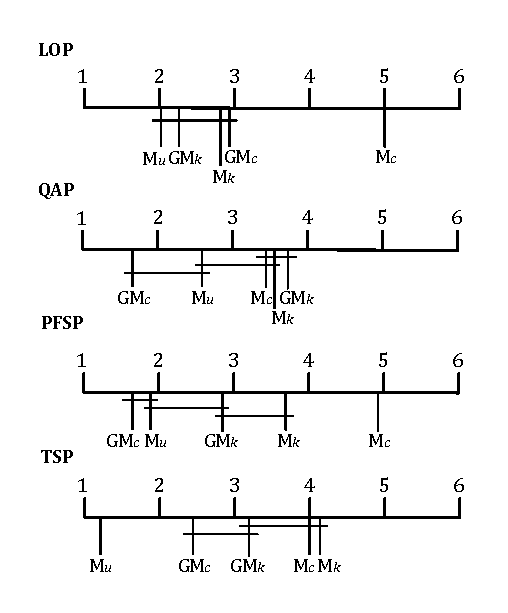
\includegraphics[width=7.5cm]{figures/critical_differences}
\end{center}
\caption{Critical difference ranking diagrams of the results.} 
\label{fig:criticaldifferences}
\end{figure}

The statistical analysis reveals that, except for the TSP, there is not just one algorithm that performs the best in the problems. However, critical difference diagrams show that $M_u$ is the most stable algorithm, being always ranked first or second. Alternatively, $M_k$ and $M_c$ are the algorithms that behave the worst, especially $M_c$.
In addition, the test shows that in the particular case of the PFSP the EDAs have very different behaviours, finding 7 pairwise comparisons statistically different out of 10. Inversely, in the LOP the algorithms performed similarly, with only four comparisons being statistically significant. As a final remark, it is worth mentioning that GMM outperforms MM, when using the same metric, almost systematically.

\section{Conclusions \& Future Work}\label{sec:conclusions}
In this paper we extend the use of Mallows and Generalized Mallows distance-based ranking models, in estimation of distribution algorithms. Beyond the commonly used Kendall's-$\tau$ distance, two new distance metrics, Cayley and Ulam, have been introduced. In order to analyse their performance when solving permutation-based combinatorial optimisation problems, a benchmark of 120 instances of four well known problems was proposed. 

The conducted experiments demonstrated that there is not just one EDA that always performs the best. However, the statistical analysis revealed that $M_u$ is the most stable EDA among the compared approaches. Alternatively, the results confirmed that Generalized Mallows EDAs are preferred to the Mallows EDAs under the same distance, which is quite obvious taking into account that GMM uses $n$ parameters to calculate the probability distribution, and the MM only 2.

As future work, there are many trends that deserve further study. On the one hand, the experimental study showed that the newly introduced Cayley and Ulam distances are able to outperform the Kendall's-$\tau$-based EDAs. Particularly, $M_u$ is the most competitive proposal for the LOP and the TSP, while $GM_c$ is preferred for the QAP and the PFSP. We think that the outstanding performance of these two EDAs could be motivated by the number of permutations that Cayley and Ulam consider at a given distance, being significantly larger than for Kendall's-$\tau$. This aspect could influence the exploration/exploration abilities of the EDA.

On the other hand, as investigated in~\cite{Echegoyen2013}, it could be interesting to analyze the relation between Mallows and Generalized Mallows EDAs, and the neighborhood system induced by the distance metrics studied in this paper.

Finally, taking into account the large performance variations observed for the studied algorithms, new EDA solutions that combine different distance metrics during the search should be investigated. %In addition, further research on optimising the classical EDA settings and specific methods for estimating $\sigma_0$ could improve the performance of the studied algorithms.

% trigger a \newpage just before the given reference
% number - used to balance the columns on the last page
% adjust value as needed - may need to be readjusted if
% the document is modified later
%\IEEEtriggeratref{8}
% The "triggered" command can be changed if desired:
%\IEEEtriggercmd{\enlargethispage{-5in}}

% references section
% NOTE: BibTeX documentation can be easily obtained at:
% http://www.ctan.org/tex-archive/biblio/bibtex/contrib/doc/

% can use a bibliography generated by BibTeX as a .bbl file
% standard IEEE bibliography style from:
% http://www.ctan.org/tex-archive/macros/latex/contrib/supported/IEEEtran/testflow/bibtex
%\bibliographystyle{IEEEtran.bst}
% argument is your BibTeX string definitions and bibliography database(s)
%\bibliography{IEEEabrv,../bib/paper}
%
% <OR> manually copy in the resultant .bbl file
% set second argument of \begin to the number of references
% (used to reserve space for the reference number labels box)

\bibliographystyle{IEEEtran}
% argument is your BibTeX string definitions and bibliography database(s)
\bibliography{bibliography}

% that's all folks
\end{document}
